% !TeX encoding=utf8
% !TeX spellcheck = de-DE

\chapter{Applikation}

Dieses Kapitel beschreibt den Entwicklungsverlauf unserer Applikation, die zugrundeliegenden Algorithmen und Datenstrukturen, sowie das Klassenmodell und die Interaktionen zwischen den verschiedenen Applikations-Schichten.

Programmausschnitte werden  in Python-Code wiedergegeben.

\section{Algorithmus}

Der Ameisen Optimierungs-Algorithmus ist in den Grundzügen einfach. Eine gewisse Anzahl autonomer Agenten (Ameisen) bewegt sich ausgehend von einem Nest-Knoten entlang eines Graphen bis zu einem Futter-Knoten. Die Ameise muss sich bei jedem Knoten entscheiden, über welche Kante sie zum nächsten gelangen möchte. Diese Entscheidung basiert hauptsächlich auf der Menge von Pheromonen, welche sich auf dieser Kante befinden. Dies wird wiederholt, bis die Ameise den Futterknoten erreicht. Danach befindet sie sich auf dem Rückweg zum Nest. Sie geht denselben Weg, den sie gekommen ist zurück und erhöht jeweils die Pheromonwerte auf den Kanten, die sie benutzt. Wenn sie das Nest erreicht hat, wird sie erneut auf den Weg geschickt.

Programmiert könnte der Algorithmus etwa so aussehen:

\begin{lstlisting}
	def ant_algorithm(ants, graph):
		for ant in ants:
			next_edge = choose_next_edge(ant.node, graph)
			ant.node = next_edge.other_node(ant.node)
			if ant.has_solution:
				ant.update_phermone_trail(next_edge)	
		evaporate_pheromones(graph)
		reset_ants_with_solution(ants)
\end{lstlisting}

Wichtig sind natürlich die verschiedenen Funktionen, die in diesem kurzen Codeblock aufgerufen werden:

\begin{description}
\item[choose\_next\_edge] Bestimmt auf der Grundlage von verschiedenen Parametern, die wir jetzt noch nicht kennen, welche Kante die Ameise als nächstes besuchen wird.
\item[update\_pheromone\_trail] Wird 
\end{description}

\section{Aufbau/Überblick}

Die Applikation besteht hauptsächlich aus zwei unterschiedlichen voneinander losgelösten Teilen: dem Benutzerinterface (GUI) und der Simulation (Backend).

Die Simulation kennt dabei die GUI-Schicht nicht, sondern wird von ihr angesprochen, wenn weitere Schritte des Algorithmus berechnet werden sollen.

TODO: Abbildung mit den zwei Teilen

\section{Vorgehen bei der Programmierung}

Wie unseren Release-Zusammenfassungen zu entnehmen ist, haben wir uns am Anfang primär auf die Entwicklung einer lauffähigen Version mit graphischer Darstellung konzentriert, in der sich Ameisen nach gewissen Regeln fortbewegen. 

\section{Mockups}

Zwei verschiedene Varianten für das spätere Aussehen des Programms standen im Vordergrund: eine mit der Einstellungsleiste im oberen Fensterbereich, eine zweite mit den Einstellungen am rechten Seitenrand.

\begin{figure}[h]
  \centering
	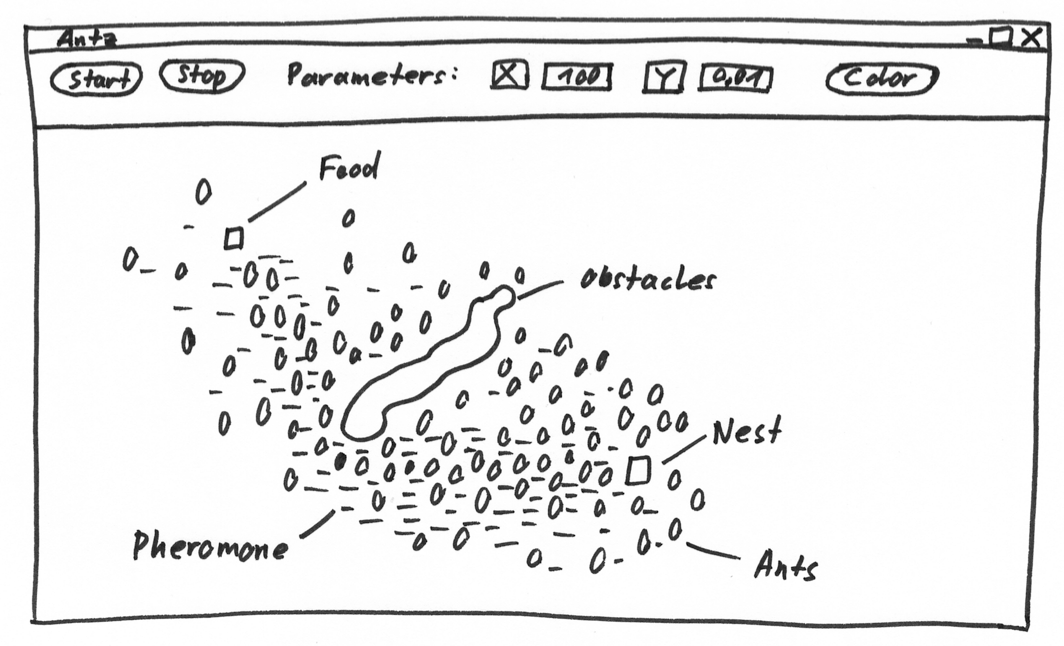
\includegraphics [width=0.85\textwidth]{images/Antz_Mockup_1_sw.png} 
	\caption{Mockup-Variante 1: Einstellungen im oberen Fensterbereich}
\end{figure}

\begin{figure}[h]
  \centering
	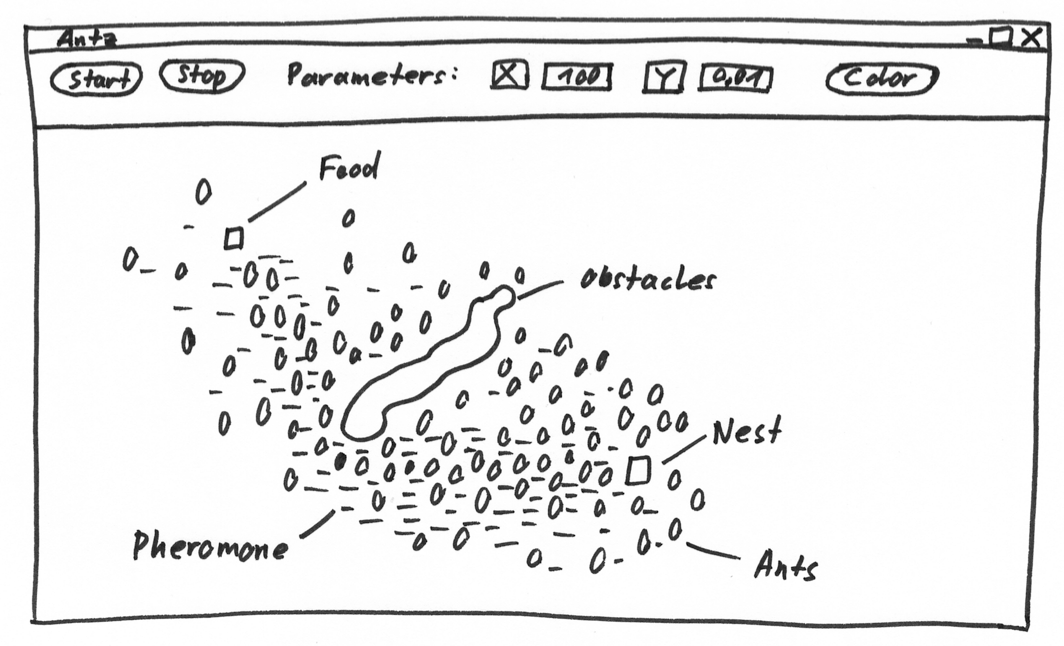
\includegraphics [width=0.85\textwidth]{images/Antz_Mockup_1_sw.png} 
	\caption{Mockup-Variante 2: Einstellungen im rechten Fensterbereich}
\end{figure}

\section{Klassendiagramme}

\section{Auswertungen: Konvergenz, Parameter}

\section{Vergleich mit Dijkstra und A*}

Wir selbst haben zwar keinen Vergleich mit Dijkstra oder A* aufgestellt, trotzdem möchten wir kurz darauf eingeben und dafür die Resultate von \citet*{leo-perf} eingehen.

\citeauthor*{leo-perf} untersucht die drei Algorithmen Dijstra, A* und Ant auf ihre Effizienz beim Finden eines kürzesten Pfades. Dabei gelangt er zu folgenden Resultaten:

\begin{table}[h]
\begin{tabular}{ | l | r | }
\hline
Dijstra & ~140ms \\
\hline
A* & ~110ms \\
\hline
Ant & ~13900ms \\
\hline
\end{tabular}
\caption{Vergleich zwischen Dijkstra, A* und Ant}
\end{table}

Man kann klar erkennen, dass der Ameisen Optimierungs-Algorithmus für die Pfadfindung nicht besonders gut geeignet ist. Zu der höheren Ausführungszeit kommt noch, dass Dijstra und A* immer den optimalen Weg finden, der Ant-Algorithmus jedoch nicht zwingend.

\citeauthor*{leo-perf} untersucht auch die Eignung des Ant-Algorithmus für das Travelling Salesman Problem und gelangt dabei zu ähnlichen Ergebnissen.

\section{Screenshots}

\subsubsection*{Iteration 1}

Noch nicht implementiert, dass die Wegfindung abhängig von der Anzahl Ameisen, die durchlaufen, ist. \\

Evtl. noch eine Multi-Threaded-Lösung integrieren (sehr gut zu parallelisieren) \\

Ausserdem: schnellere Python-Interpreter wie pypy (oder für numerische Berechnungen); für z.B . 10'000 Nodes! \\

Idee: vielleicht noch Rauschen integrieren? Random von 20\,\% konvergiert überhaupt nicht mehr.

\vspace*{3cm}


Inputs von Syrus: \\

\begin{itemize}
\item Interessant wäre, das Maximum der Verlangsamung bei mehr Ameisen zu messen
\item Eventuell in Richtung Programming Tuning gehen? (Performance-Messungen: wie viel fällt auf welchen Bereich?) 
\item Für die Iterationen 2 und 3: Einsatz der Ressourcen planen (Andere Algorithmen; Optimierung; Vergleich mit Djikstra: Statistiken; vgl. Optimierungspotential bezüglich Zeit und Speicheraufwand, etc.); z.B. eher TSP (weil visuell für die Mitstudierenden ansprechender?) 
\end{itemize}